\documentclass{article}

\usepackage{amsmath}
\usepackage{graphicx}

\addtolength{\oddsidemargin}{-.3in}
\addtolength{\evensidemargin}{-.3in}
\addtolength{\textwidth}{0.6in}

\begin{document}

\title{Homework 6\\
       OpenMP}
\author{Geoffrey Ulman\\
        CSI702}
\date{April 2010}
\maketitle

\section{Design}
Because generation of the Mandelbrot set is a truly embarrissingly parallel problem, using OpenMP to parallelize the serial code was very simple. At the core of the serial code are two nested loops which iterate through the columns and rows of the discretized Mandelbrot set grid. Because calculating a single row (the inner loop) is a relative fast operation and there are many more rows (typically 512 or 1024 in the experiments performed) than the number of available processors (typically 2 to 8 in the experiments performed), parallelizing the outer loop and performing the inner loop iterations in serial was enough to keep all available processors busy in most cases.

\section{Challenges}


\section{OpenMP Commands}
The standard \verb!#pragma omp parallel for! directive was used in front of the outer for loop in the Mandelbrot calculation. The shared and private variables were specified using \verb!default(shared)! and \verb!private(i,j,x,y,zr,zi,it,zr2,zi2)!. To facilitate performing multiple test runs without recompiling, \verb!schedule(runtime)! was used and scheduling was set using the \verb!OMP_SCHEDULE! environment variable. The number of threads used was set using the \verb!OMP_NUM_THREADS! enviroment variable.

\section{Performance Analysis}

Performance tests were performed on three different computer systems: an 8 core Ubuntu box using 2.33GHz Intel Xeon CPUs hosted on Amazon EC2, a 2 core node on the GMU cds cluster, and an 8 core node on the GMU gmice cluster. In each case tests were performed varying the problem size, number of threads, and thread scheduling techniques.

Figure \ref{amazon_n} demonstrate the effect of increasing problem size on the 8 core Amazon EC2 node. For all problem sizes, the parallel OpenMP code used static scheduling with a chunk size of 10. The most striking observation from these results is the sharp dropoff in speedup as the probem size (the number of rows or columns in the discretized Mandelbrot set) falls below 1024. Presumably using OpenMP adds some amount of overhead to the code as threads must be created and destroyed (there should be no synchronization overhead in this code). That overhead might begin to overwhelm the performance gains due to multithreading for small problem sizes. However, this is hard to believe due to the lightweight nature of threads (creating and destroying them is a very fast operation). The other possible explanation for the performance dropoff is that the ratio of chunk size to total problem size becomes larger and larger as the total problem size shrinks. This makes it more likely that one thread could be assigned a particularly computationally intensive portion of the Mandelbrot set.

\begin{figure}
\centering
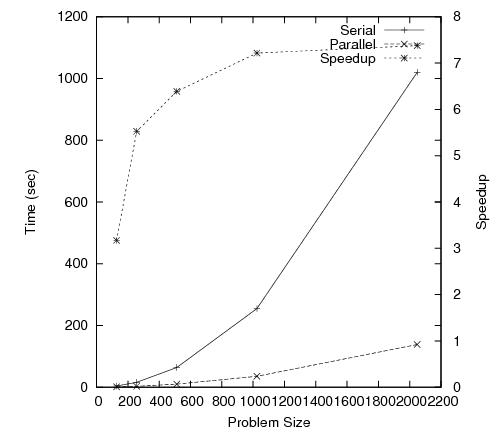
\includegraphics[width=0.7\textwidth]{../data/amazon_n.png}
\caption{Parallel and Serial Timing Results on Amazon EC2 Node with 8 Threads and Static,10 Scheduling and Variable Problem Size}
\label{amazon_n}
\end{figure}

\begin{figure}
\centering
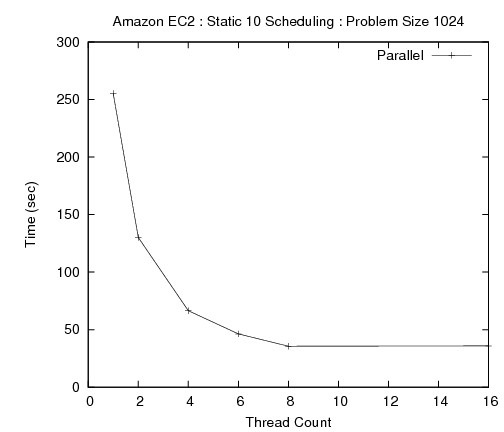
\includegraphics[width=0.7\textwidth]{../data/amazon_threads.png}
\caption{Parallel Timing Results on Amazon EC2 Node with 1024 Problem Size and Static,10 Scheduling and Variable Thread Count}
\label{amazon_threads}
\end{figure}

\begin{figure}
\centering
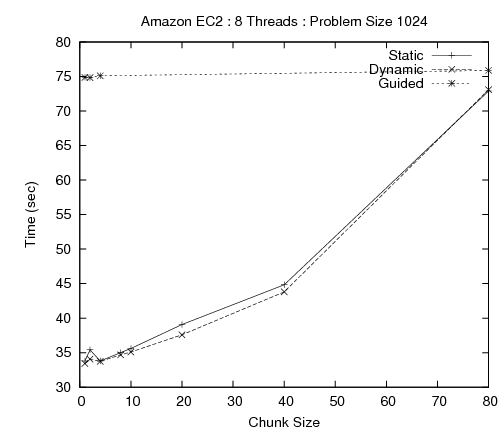
\includegraphics[width=0.7\textwidth]{../data/amazon_chunk.png}
\caption{Parallel Timing Results on Amazon EC2 Node with 1024 Problem Size and 8 Threads and Variable Scheduling}
\label{amazon_chunk}
\end{figure}







\begin{figure}
\centering
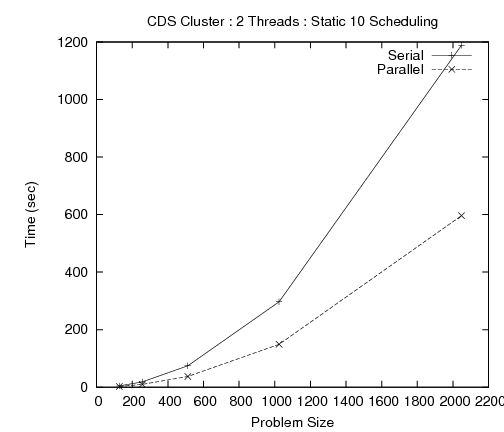
\includegraphics[width=0.7\textwidth]{../data/cds_n.png}
\caption{Parallel and Serial Timing Results on CDS Node with 8 Threads and Static,10 Scheduling and Variable Problem Size}
\label{cds_n}
\end{figure}

\begin{figure}
\centering
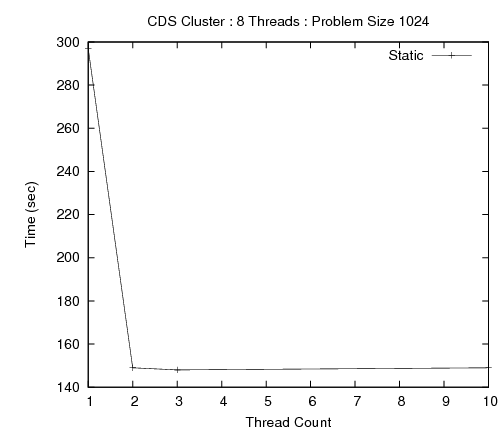
\includegraphics[width=0.7\textwidth]{../data/cds_threads.png}
\caption{Parallel Timing Results on CDS Node with 1024 Problem Size and Static,10 Scheduling and Variable Thread Count}
\label{cds_threads}
\end{figure}

\begin{figure}
\centering
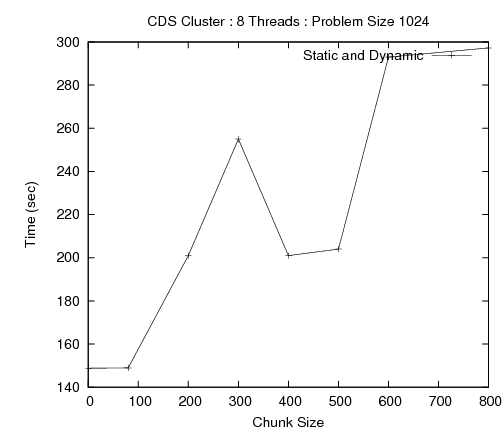
\includegraphics[width=0.7\textwidth]{../data/cds_block.png}
\caption{Parallel Timing Results on Amazon EC2 Node with 1024 Problem Size and 8 Threads and Variable Scheduling}
\label{cds_chunk}
\end{figure}




\section{Output Comparison}
\label{outputcomp}

\begin{thebibliography}{9}

\bibitem{cpl}
  Brian W. Kernighan and Dennis M. Ritchie,
  \emph{The C Programming Language},
  Prentice Hall PTR, New Jersey,
  2009.

\end{thebibliography}

\end{document}
